\documentclass[11pt]{article}

\usepackage{fullpage}
\usepackage{color}
\newcommand{\BKM}[1]{\textcolor{blue}{BKM: #1}}
\newcommand{\RNG}[1]{\textcolor{red}{RNG: #1}}

\usepackage[export]{adjustbox}
\usepackage{fancyhdr}
\pagestyle{fancy}
\fancyhf{}
\rfoot{\thepage}
\cfoot{
\includegraphics[height=0.6in,valign=c]{LetterheadFooter}}
\renewcommand{\headrulewidth}{0pt}

\newenvironment{response}
{\begin{quote}\itshape}
{\end{quote}}

\setlength{\parindent}{0em}
\setlength{\parskip}{0.5em}

\usepackage{xr}
\externaldocument{NAR_DRAFT}

\begin{document}
\vspace*{-0.5in}\hspace*{-0.2in}
\includegraphics{LetterheadHeader}\vspace*{\baselineskip}

\noindent Dear Professor Herrero,

We appreciate the opportunity to revise our manuscript for publication in \emph{NAR Genomics and Bioinformatics}, and we thank you and the reviewers for the quality of the reviews. Below we respond in italics to the reviewers' concerns.

\noindent Sincerely,\\
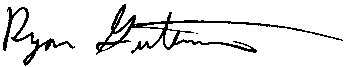
\includegraphics{signature}\\
Ryan Gutenkunst, PhD\\
Associate Professor and Associate Department Head\\
Department of Molecular and Cellular Biology\\
University of Arizona

\section*{Associate Editor}

Stressing on some of the points raised by the reviewers, I would suggest you include more details about the assumption and limitations of BATCAVE. In particular, the possibility of changes of mutational signatures over time can be quite striking in some cases, especially if the original tumour is driven by very specific mutagens like UV light or tobacco smoke. Ideally, the software should try to correct for these cases or at least warn the user about a possible shift in signatures/contexts.
\begin{response}
\RNG{Correcting for context shifts beyond the scope of the current manuscript. But warning about it is a very good idea. Simple check, do a goodness-of-fit test on called the low-confidence mutations. What is the p-value for their profile versus the high-confidence? (A $\chi^2$ test may not be appropriate here, since many entries may have small numbers. This preprint suggests potential improvements: https://arxiv.org/abs/1711.05524.)}
\BKM{This looks quite easy to implement. Testing is another question. One thing we don't have right now is simulations where the signature changes appreciably, but we do have the infrastructure to do it.}
\end{response}

Related to this, there is probably a minimum number of high-confidence mutations that are required by BATCAVE to produce reliable results. As with the previous point, ideally the batcaver should address or warn the user if the assumptions are violated.
\begin{response}
\RNG{Good idea, should be an easy check. Easiest way would be to count high-confidence mutations. More sophisticated approach would be to evaluate the convergence of the prior, using something like K-L distance.}
\BKM{This makes sense to me. We could pick some sensible threshold and note the allele frequency at which it is crossed.}
\end{response}

Lastly, as correctly pointed out by the second reviewer, the sequencing coverage only makes sense in the context of the purity of the samples and this information should be provided to the reader.
\begin{response}
\RNG{Brian: Can you think about this in the context of what MuTect already does?}
\BKM{Mutect has a parameter for contamination/purity if known. I could add a parameter default=0, and write a message to stdout with the value used. There are various methods for estimating purity.}
\end{response}


\section*{Reviewer 1}

Mannakee and Gutenkunst present BATCAVE, an algorithm that first estimates the tumor’s mutation profile and mutation rate using high-confidence variants and then uses them as a prior when calling other variants based on mutational signatures. The concept behind this work is interesting. However, the difference in accuracy between MuTect and BATCAVE is relatively small except for the case when one has particularly high depth sequencing (500x), limiting the utility of the method. 

Still, the 500x whole exome case does indicate that BATCAVE is better at identifying low frequency variants and thus can better reveal intratumoral heterogeneity, an important area of inquiry in cancer. Interestingly, the AUROC values for both MuTect and BATCAVE have room for improvement for the 500x whole exome case (Table 1). I suggest the authors further investigate how to improve the AUROC values. For example, in equation 4, it is unclear why the authors assume $\nu$ be uniformly distributed. Although this is also an assumption of MuTect, the BATCAVE approach inherently distinguishes mutations by allele frequency – since log-likelihood is closely associated to AF.  Perhaps a model in which $\nu$ follows a decreasing distribution vs. AF (e.g. in concordance with a model of a growing tumor) would yield better AUROC values.  
\begin{response}
\RNG{We've thought about this... Didn't we decide that it didn't make sense, because we'd just be overweighting low-frequency variants? I can think more about it.}
\BKM{We thought about it and I actually implemented a version. What happened is that for the distribution I think is indicated the correction was far too strong, like you said it overweights low frequency variants. I will also think about ways to do this.}
\end{response}

In Rubanova et al ( https://www.biorxiv.org/content/10.1101/260471v4.full), it is argued that there are changes in mutational signatures over time in cancers. While Mannakee and Gutenkunst mention this work, they should further comment on whether such changes in mutational signatures over time are small enough to be explained by the BATCAVER concept of re-evaluating mutations based on p-value.
\begin{response}
\RNG{Going to be difficult, depending on biology to offer specific guidance about the size of the change. Rather, we now do a goodness-of-fit test and warn the user if it looks like it's violated.}
\BKM{We could detect a change above. Whether it matters or not is a complex interplay between depth and selection. For late changes most mutations with that signature will be below the threshold of detection. For an early mutation all of the marginal (low frequency) variants will be from the signature.}
\end{response}

Minor
p.2: “Folding the central base to the pyrimidines”: The “folding” terminology is not standard and should be improved. 
\begin{response}
Corrected
\end{response}

Equation 11: This equation is not correct if there is subclonal copy number evolution that changes the distribution of mutations above the allele frequency threshold. The authors should more clearly state this assumption.
\begin{response}
\RNG{Revise to include assumption, and think in general about copy number changes. How does a standard MuTect pipeline handle this?}
\BKM{Will do. MuTect doesn't make copy number calls, and doesn't adjust allele frequency I don't think. They basically ignore it. I think a change large enough to have a real effect here would be more of a change in ploidy.}
\end{response}

\section*{Reviewer 2}

Mannakee et al have developed a tool called BATCAVE for calling mutations from sequencing data. They claim to have used a novel approach of using tumor and site-specific priors for calling mutations. In my opinion authors have done a good job in terms of using a novel approach which harnesses patient/tumor specific information to call mutations. I agree with the authors that this approach was missing in other tools. I accept this study to be published given the authors address few points mentioned below:

1. Does BATCAVE accounts for tumor purity estimates while calling mutations?
\begin{response}
\RNG{Brian: How does MuTect handle this?}
\BKM{We do not. MuTect has a parameter for this, I will check exactly what it does.}
\end{response}

2. In case of multi-region sequencing data, used for studying spatial intra-tumor heterogeneity, usually the existing tools estimate very high levels of heterogeneity. I suppose this is because they are being very stringent in terms of calling mutations especially the ones with low vafs. In that case the people end up using other tools like bamreadcount etc. to check status of these mutations in the bam files and re-estimate the extent of heterogeneity. It will be important to see how BATCAVE performs in such datasets.
\begin{response}
\RNG{Unclear to me whether we should dodge this. We could say explicitly accounting for multiregional samples is out-of-scope, and add it to the discussion. Although we did do something like that for our breast cancer analysis.}
\BKM{One of the reasons we made the algorithm is to try to provide a more sensitive means for identifying low frequency alleles so that these types of measures are more accurate. The multi-region sample we got simply isn't deep enough for us to figure out whether we would change the heterogeneity calls. There are not enough callable low frequency variants. Which is why our performance is identical. I am unaware of any deeper data sets, and think simulating them is beyond the scope.}
\end{response}

3. Do the mutation signatures (example smoking signatures in lung cancer or UV signatures in melanoma) still appear in the more stringent BATCAVE set of mutations?
\begin{response}
\RNG{Not exactly sure what the reviewer is asking here, but should be easy to check. It will certainly still appear in simulations. Not sure about the real data analyses. But we can check when we add our test as to whether the distribution has changed.}
\BKM{I am not entirely sure. Perhaps he is asking if we decomposed the final "prior" multinomial parameters to see if we get the same signatures back out? We don't because as we observed in the work I was doing with Setayesh that the tools like deconstructSigs are bad. We know that we converge to the simulated distribution and we know that the simulated distribution is a equal linear combination of the 3 signatures we describe.}
\end{response}

\end{document}
